% Source : http://tex.stackexchange.com/questions/34382/tikzpicture-has-a-node-whose-text-is-a-tree-unevenly-formatting

\documentclass{minimal}
    \usepackage{tikz}
    \usetikzlibrary{chains}


\begin{document}

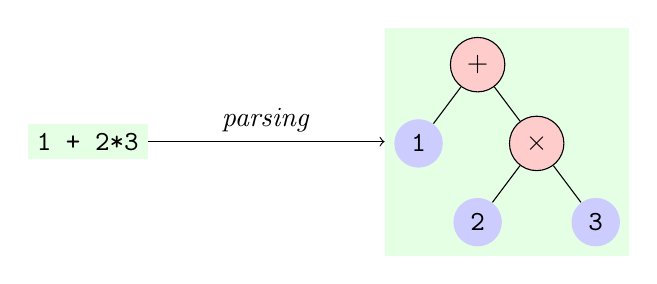
\begin{tikzpicture}[
    level distance=10mm,
    op/.style={circle,draw,fill=red!20},
    leaf/.style={circle,fill=blue!20,font=\ttfamily},
]
    \node (out) [fill=green!10] {
        \tikz{
            \node [op] {$+$}
            child { node [leaf] {1} }
            child { node [op] {$\times$}
            child { node [leaf] {2} }
            child { node [leaf] {3} }};
        }
    };
    \node (in) [fill=green!10,left=30mm of out] {\texttt{1 + 2*3}};
    \draw[->] (in) -- node [above] {\emph{parsing}} (out);
\end{tikzpicture}

\end{document}
